\section{Question 2}

\begin{question}
    Solve $$\left\{\begin{array}{l}-\Delta u=f, \text { in } \Omega \\ \left.u\right|_{\Gamma_1}=g_1,\left.\frac{\partial u}{\partial \vec{n}}\right|_{\Gamma_2}=g_2\end{array}\right.$$
    with a piecewise linear continuous FEM. Describe your method clearly and write down the resulted linear system with every entry of the matrix and vectors clearly defined, indicating the zeros. Show that the linear system has a unique solution.
    
    From Figure \ref{fig:fig1}, $\vec{n}$ is the outward pointing unit normal vector. Use the provided mesh for your FEM.
    
    \begin{figure}[H]
        \centering
        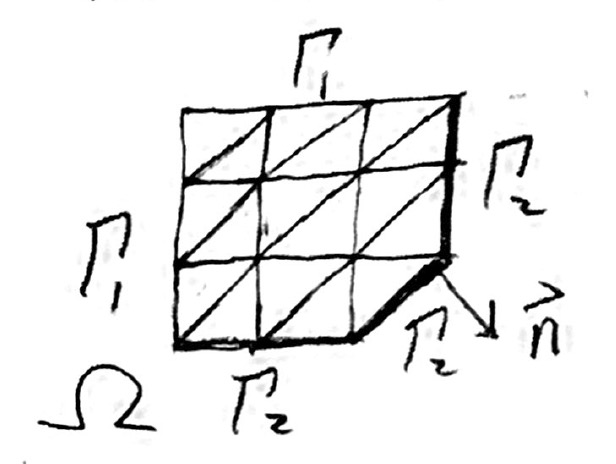
\includegraphics[width=0.3\textwidth]{Figure1.jpeg}
        \caption{\label{fig:fig1}Provided Mesh for Question 2}
    \end{figure}
\end{question}

\begin{answer}
    
\end{answer}